%%%%%%%%%%%%%%%%%%%%%%%%%%%%%%%%%%%%%%%%%%%%%%%%%%%%%%%%%%%%%%%%%%%%%%%%%%%%%%%%
\glsresetall
\section{Introduction}
As more of society becomes integrated with \gls{ml}, bias, fairness, and the formalization of \gls{ml} standards are topics of high interest ~\cite{10.1007/978-3-030-13469-3_68, anne2018women, wang2018racial}. One effect of the growing dependency on technology is the increasing concern regarding biased and unfair algorithms.  For instance, \gls{fr} systems can be untrustworthy and racist in some cases~\cite{england2019,snow2018}.
. 

\begin{figure}[t!]
\centering
         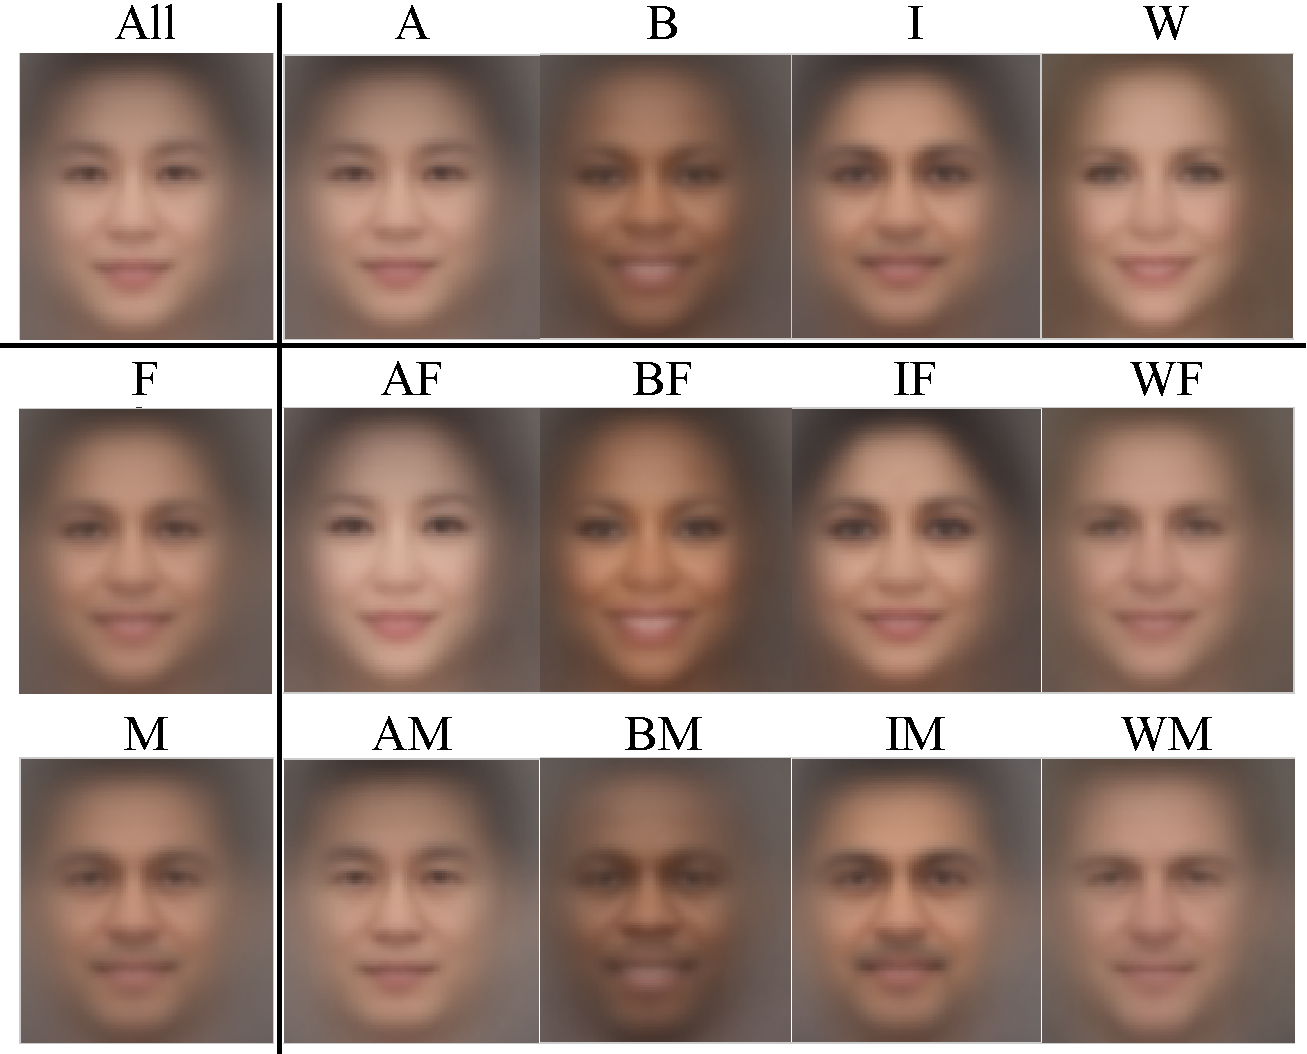
\includegraphics[width=\linewidth]{figures/montage.pdf}
\caption{\textbf{\gls{bfw}.} The average face of its different subsets: \emph{top-left}: the entire \gls{bfw}; \emph{top-row} per race;  \emph{left-column}: per gender. The others represent the ethnicity and gender of the race and gender, respectfully. Table~\ref{tab:ethnic-splits} defines the acronyms of subgroups.}
\label{fig:avg-faces}
\end{figure}

Typically, \glspl{cnn} are trained on faces identified by a detection system. Specifically, for \gls{fr}, the goal is to project faces to an N-dimensional space with minimal distances between samples of the same identity and maximize the gap separating those that are different. Thus, the overarching goal is to discriminate between subjects with face encodings. We can deploy such a \gls{cnn} to encode faces to compare via a similarity score: genuine pair if the score is high enough; and rejected as an imposter. 

A fixed threshold acts as a decision boundary in similarity score space. Thus, the face features in the same class must satisfy a criterion in the form of a single value~\cite{deng2019arcface, liu2017sphereface, wang2018additive, wang2018cosface}. However, a single, global threshold is a crude measure that leads to \gls{fr} errors. Furthermore, the held-out set used to determine the global threshold tends to share the same distribution with test data, which makes the results skewed in favor of specific demographics that make up a majority in both sets. That skew, the difference in the performance of an algorithm of certain ethnic groups, is our definition of bias. A key question is: \emph{is \gls{fr} too biased, or not?} 


\begin{table*}[t!]
\scriptsize
    \centering
       \caption{\textbf{The proposed \gls{bfw} compared to related datasets.} \gls{bfw} is exactly balanced across ID, gender, and ethnicity (Table~\ref{tab:ethnic-splits}). Compared with \gls{dp}, \gls{bfw} provides more samples per subject and subgroups per set. Also, \gls{bfw} uses a single resource, VGG2. \gls{rfw}, on the other hand, supports a different task (\ie domain adaptation). Furthermore, \gls{rfw} focuses on race-distribution across of pairs, while not considering the distribution of identities. }
    \begin{tabular}{rccccccc}%x{10mm}x{3mm}x{10mm}x{8mm}}%\toprule
    
    \multicolumn{2}{c}{Database} & \multicolumn{3}{c}{Number of}& \multicolumn{3}{c}{Balanced Labels}\\
    \cmidrule(lr){1-2}	\cmidrule(lr){3-5} \cmidrule(lr){6-8}
    Name & Source Data & Faces &  IDs & Subgroups & ID & Ethnicity & Gender\\\midrule
    \gls{dp}~\cite{demogPairs}     & CASIA-W, VGG\&VGG2 & 10,800& 600 & 6 &\checkc& \checkc &\checkc \\
    \gls{rfw}~\cite{wang2018racial}     &  MS-Celeb-1M &$\approx$80,000&$\approx$12,000& 4 & \xmark & \checkc &\xmark \\
    \gls{bfw} (ours) & VGG2 & 20,000 & 800 &8 & \checkc & \checkc &\checkc \\\bottomrule
    \end{tabular}
    \label{tab:compared}
    % \vspace{-4mm}
\end{table*}

The adverse effects of a global threshold are two-fold: \textbf{(1)} the mapping produced by a \gls{cnn} is nonuniform. Therefore, distances between pairs of faces in different demographics vary in distribution of similarity scores (Fig~\ref{fig:detection-model}); \textbf{(2)} the evaluation set is imbalanced as well. Particular demographics making up a majority of the population will carry most weight on reported performance ratings. Reported results skew away from common traits to the underrepresented subgroups. Alas, demographics like gender, ethnicity, race, and age are underrepresented in most public datasets. 

Making matters more challenging is that race and ethnicity are loosely defined.  For example, the US Census Bureau allows an individual to self-identify race (\href{https://www.census.gov/mso/www/training/pdf/race-ethnicity-onepager.pdf}{https://www.census.gov}). We define it as a group of people having facial characteristics similar to those found in a region. The result is various types of biases in FR systems in favor of or against particular demographics remain a question.



To address \textbf{(2)}, the lack of a balanced data, we introduce a new benchmark for \gls{fr}, called \gls{bfw} (Table~\ref{tab:compared}, ~\ref{tab:ethnic-splits}). \gls{bfw} serves as a platform to fairly evaluate \gls{fr} systems and enable demographic-specific ratings to be reported. We use \gls{bfw} to gain a deeper understanding of the extent of bias present in facial embeddings extracted from a \gls{soa} \gls{cnn} model. We then suggest a mechanism to counter the biased feature space to mitigate problems of bias with more balanced performance ratings for different demographics, while improving the overall accuracy. Specifically, we propose using an adaptive threshold that varies depending on the characteristics of detected facial attributes (\ie gender and ethnicity, Fig~\ref{fig:avg-faces}). We show an increase in accuracy with a balanced performance for different subgroups of people. Similarly, we show the positive effect of adjusting the similarity threshold based on the facial features of matched faces. Thus, selective use of similarity thresholds in current \gls{soa} \gls{fr} systems provides more intuition in \gls{fr}-based research, while providing a method easily adoptable in practice. 


\begin{table*}[!t]
    \centering
    \caption{\small{\textbf{Database stats and nomenclature, optimal thresholds ($t_o$), and accuracy scores.} \textit{Header:} Subgroup definitions. \textit{Top-row:} Statistics of \gls{bfw}. \textit{Middle:} Number of pairs for each partition. \textit{Bottom:} Accuracy with a global threshold $t_g$, the optimal threshold $t_o$, and accuracy with $t_o$ per subgroup. Specifically, $t_g$=0.259$\pm$0.002 when averaged across the five folds. Columns grouped by race and then further split by gender. Out of millions of pairs, accuracy is inconsistent across subgroups. Furthermore, $F$ tend to perform inferior to that of $M$ for all but B.}}\label{tab:ethnic-splits}
    \scalebox{1}{
     \resizebox{\textwidth}{!}{%
    \begin{tabular}{r c c c c c c c c l}
        \toprule
        & \multicolumn{2}{c}{Asian (A)} & \multicolumn{2}{c}{Black (B)}  & \multicolumn{2}{c}{Indian (I)}& \multicolumn{2}{c}{White (W)}\\
        \cmidrule(l){2-3} \cmidrule(l){4-5} \cmidrule(l){6-7}\cmidrule(l){8-9} % spanning less than the full width of the table - you can add (r) or (l) just before the opening curly bracket to shorten the rule on the left or right side
         & Female (AF) & Male (AM) & BF & BM& IF & IM & WF & WM&Aggregated\\ % Column names row
        \midrule

       \# Faces  &  2,500&  2,500& 2,500 & 2,500& 2,500 & 2,500 & 2,500 & 2,500 &20,000 \\ % row 1
        \# Subjects & 100& 100& 100  & 100  & 100  & 100& 100 &100&800  \\ % row 2
        \# Faces / Subject  & 25 & 25    & 25 & 25 & 25  & 25  &  25 & 25 & 25\\ % row 3
        % \midrule
\specialrule{.01em}{.05em}{.05em}
            \# Positive Pairs &  30,000&  30,000& 30,000 &30,000 & 30,000 &30,000&30,000 & 30,000 &240,000 \\ % row 1
        \# Negative Pairs & 85,135&  85,232& 85,016  & 85,141  & 85,287  & 85,152& 85,223 &85,193&681,379  \\ % row 2

        \# Pairs (Total) & 115,135 & 115,232    &115016 &115,141 & 115287  & 115,152  &  115,223& 115193 & 921,379\\ % row 3
        % \midrule
        \specialrule{.01em}{.05em}{.05em}
        Acc$@t_g$ & 0.941 & 0.952  & 0.967 & 0.960 & 0.958 &0.962  & 0.973 & 0.981 &0.962 $\pm$0.012 \\
        $t_o$ & 0.255 &  0.246 & 0.277 &0.242  &0.297 & 0.264& 0.233 &0.239 &0.257$\pm$0.006\\ % row 4
        
        Acc$@t_o$ & 0.942 &0.952 &0.968 &0.961 &0.960 &0.962 & 0.974 &0.982 & 0.963 $\pm$ 0.012\\
        \bottomrule
    \end{tabular}}
    \glsunset{af}
    }
    \glsunset{af}
    \glsunset{am}
    \glsunset{bf}
    \glsunset{bm}
    \glsunset{if}
    \glsunset{im}
    \glsunset{wf}
    \glsunset{wm}
    % \vspace{-12pt}
\end{table*}




The contributions in this paper are as follows:
\begin{enumerate}
    \item Built a balanced dataset as a proxy to measure verification performance per subgroup.
    \item Analyzed an unwanted bias in scores of face pairs while showing that optimal thresholds determined per subgroup significantly boost and balances performances.
    \item Showed bias causes inconsistencies in ratings across demographics-- the typical use of a global threshold unfavorable. We mitigate the problem via adaptive thresholds.
    \item Conducted human-evaluations to demonstrate bias in human perception.\footnote{NIH-certified, \textit{Protect Humans in Research}, \textcolor{red}{IRB 19-09-08}.}
\end{enumerate}

